%\section{Empricial Experiments}

\section{Evaluating Enhanced Techniques}
\label{sec:evaluation}

This section evaluates the enhanced downstream
testing techniques on real-world subject programs
that contains test dependence.

\subsection{Subject Programs}

For each of the downstream testing techniques we studied,
we only applied our enhanced version of the technique
if the subject program and its corresponding test suite revealed
dependent tests in its nonenhanced orders. 
The subject program characteristics are shown
in Section~\ref{sec:subj}.

\subsection{Methodology}

We evaluate each testing technique in two aspects:
\begin{enumerate}
\item We apply each technique to all test suites containing
test dependence, and then check whether the test dependence
has been properly handled, i.e., no test in the output
reveals different results than being executed in the original
test suite in the default order.
\item We analyze the outcome of each enhanced,
dependence-aware testing technique, and check whether
the technique effectiveness has been compromised or not.
Specifically, for test prioritization techniques, we measure
the test coverage of the prioritized test suite. For test
selection techniques, we measure the size of the selected
test subset. For test parallelization techniques, we measure
the execution time for the whole test suite.

\end{enumerate}

%\subsubsection{Understanding Dependence Root Causes}

%results
\begin{figure}[t]
%\hspace{0.5cm}
\begin{minipage}[b]{\linewidth}
\centering
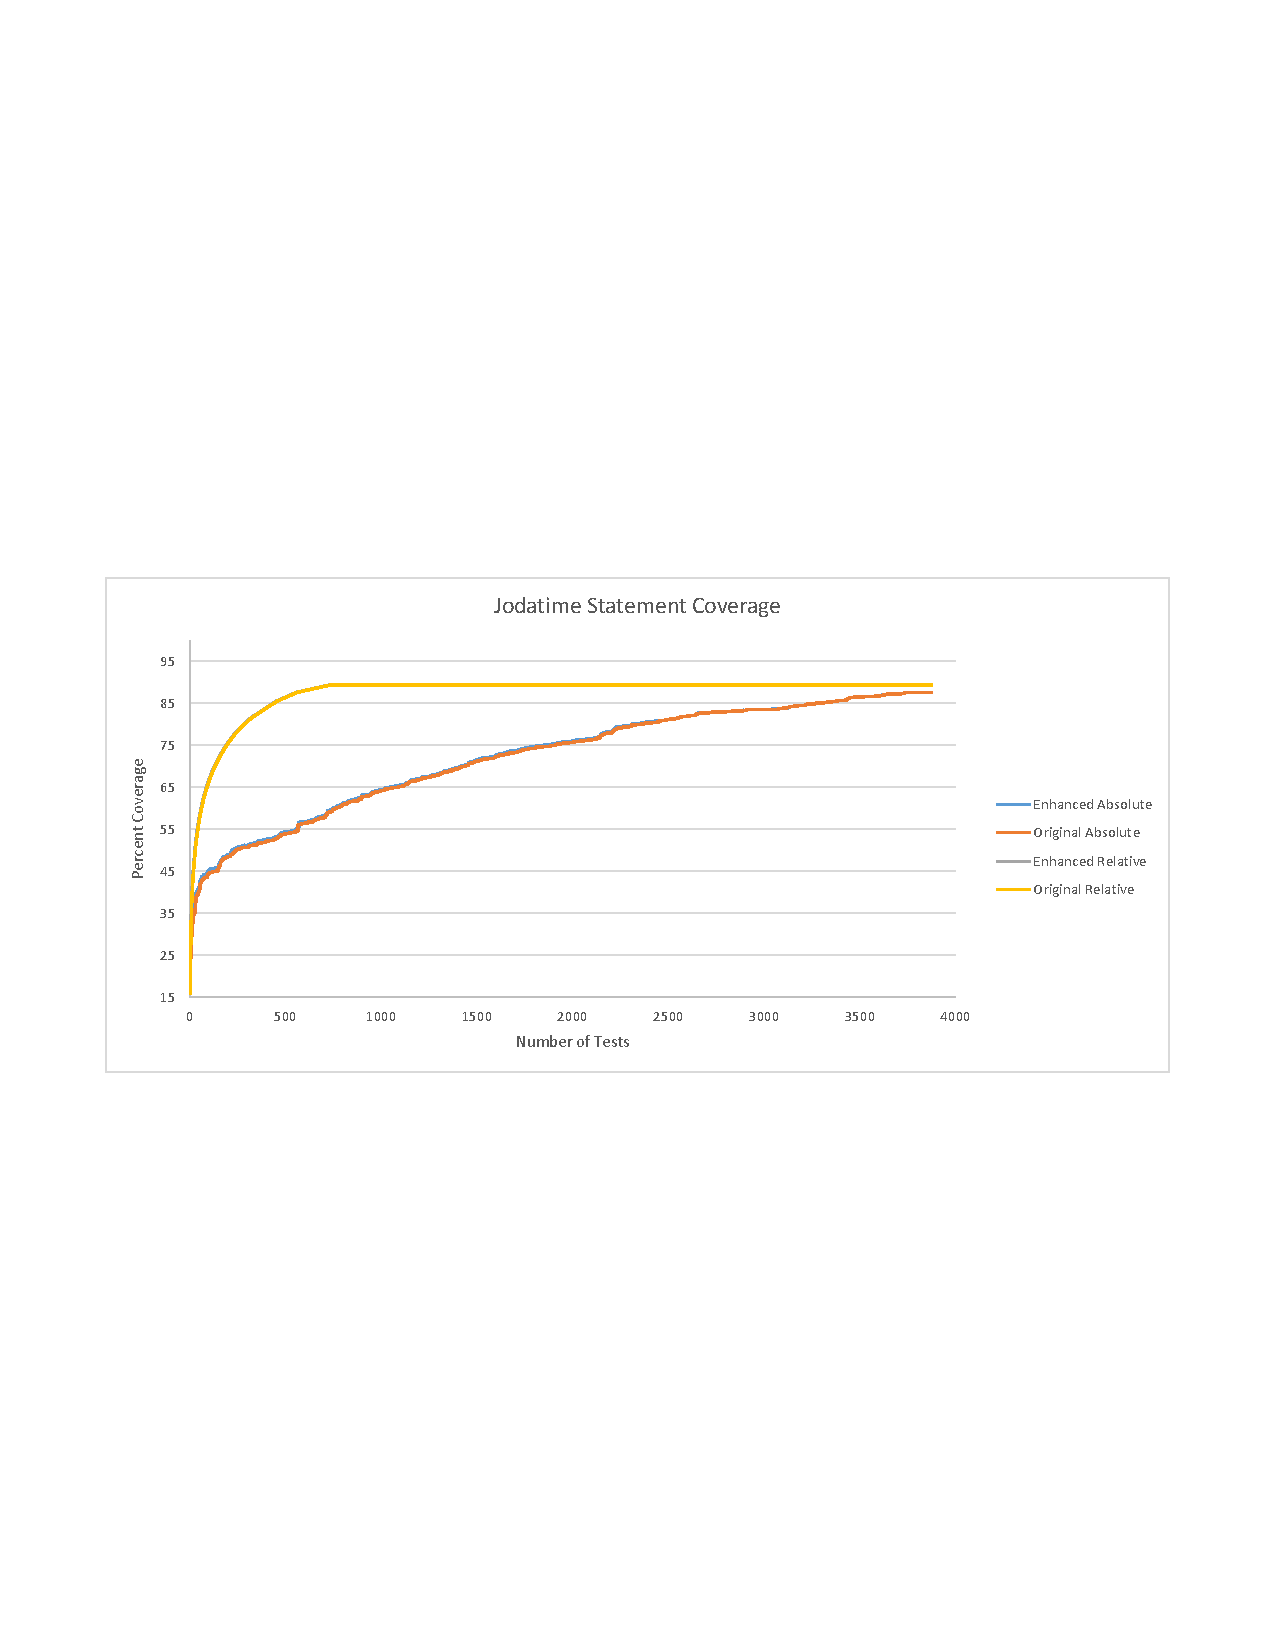
\includegraphics[scale=0.46]{jodatime-coverage-figure}
Jodatime
%\caption{replace} \label{fig:p2}
\end{minipage}
\begin{minipage}[b]{\linewidth}
\centering
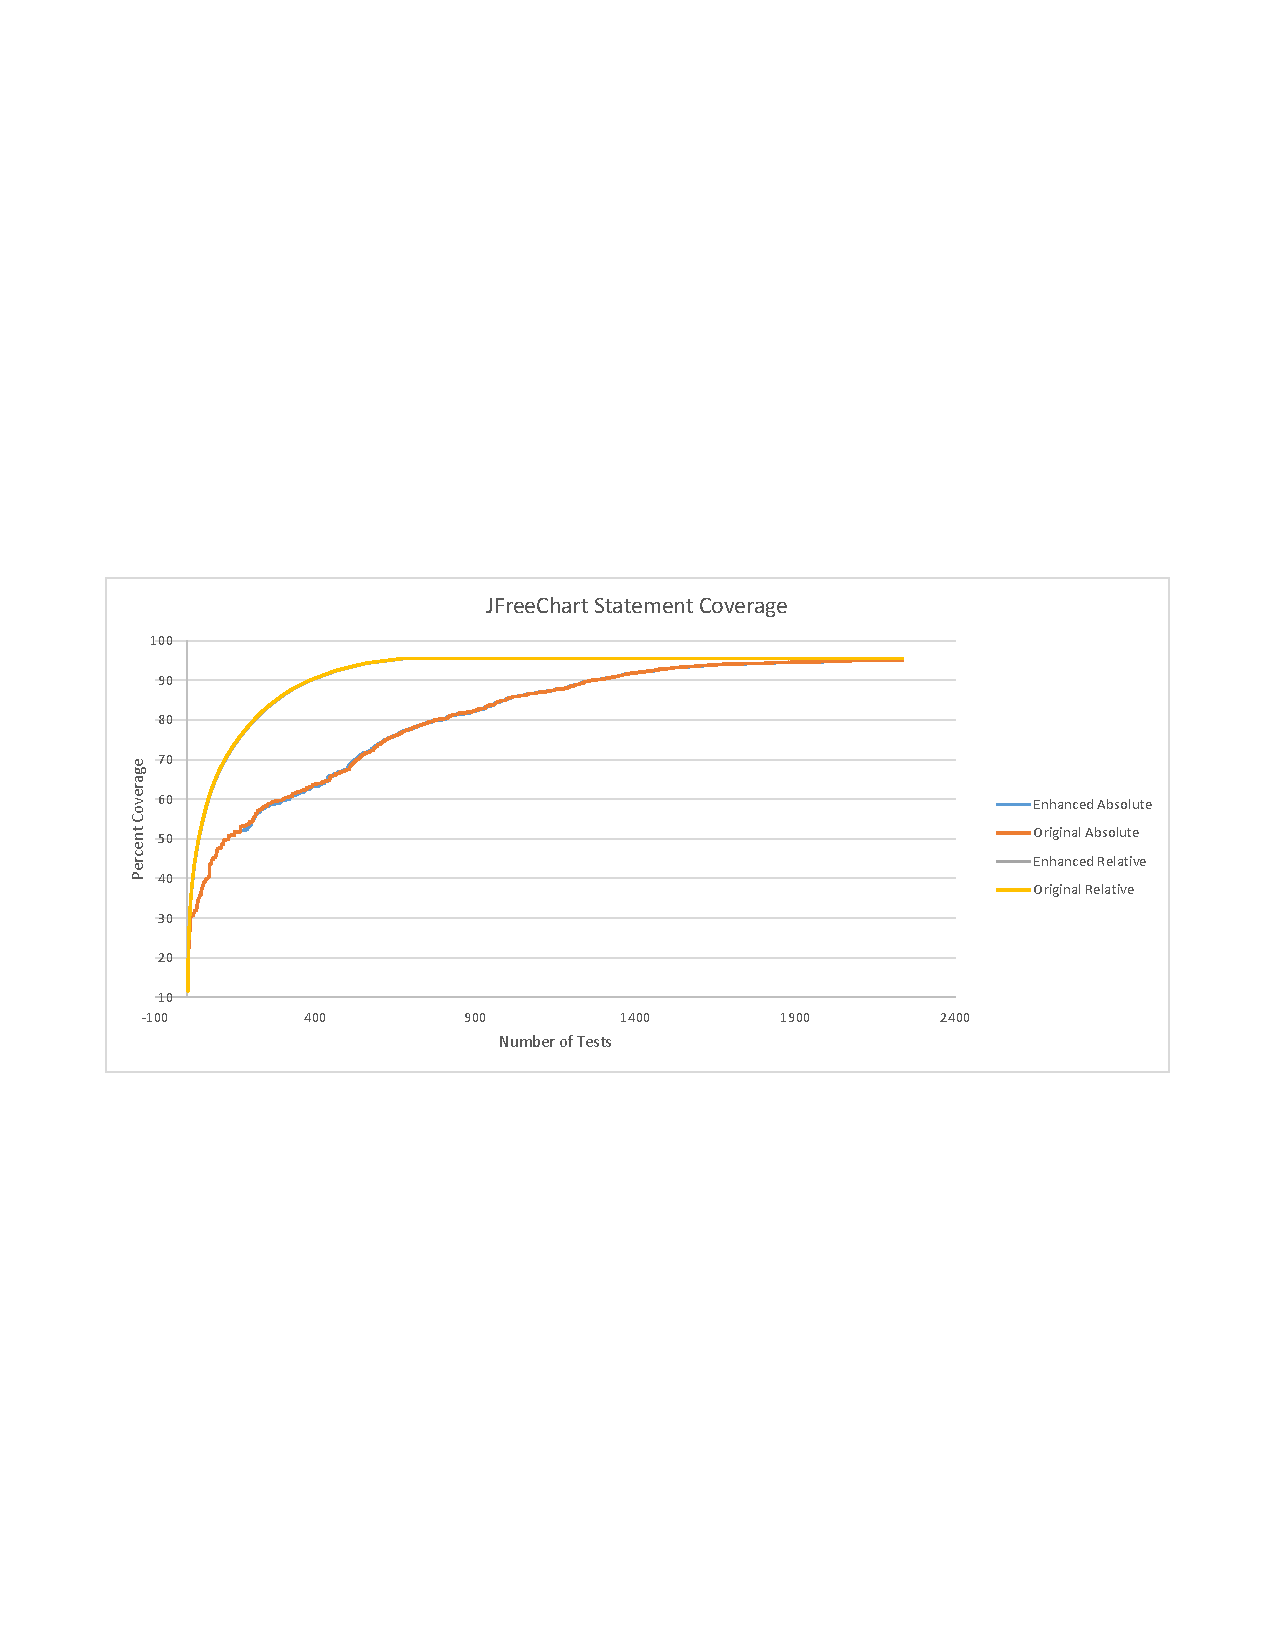
\includegraphics[scale=0.46]{jfreechart-coverage-figure}
JFreechart
%\caption{schedule} \label{fig:p3}
\end{minipage}
\begin{minipage}[b]{\linewidth}
\centering
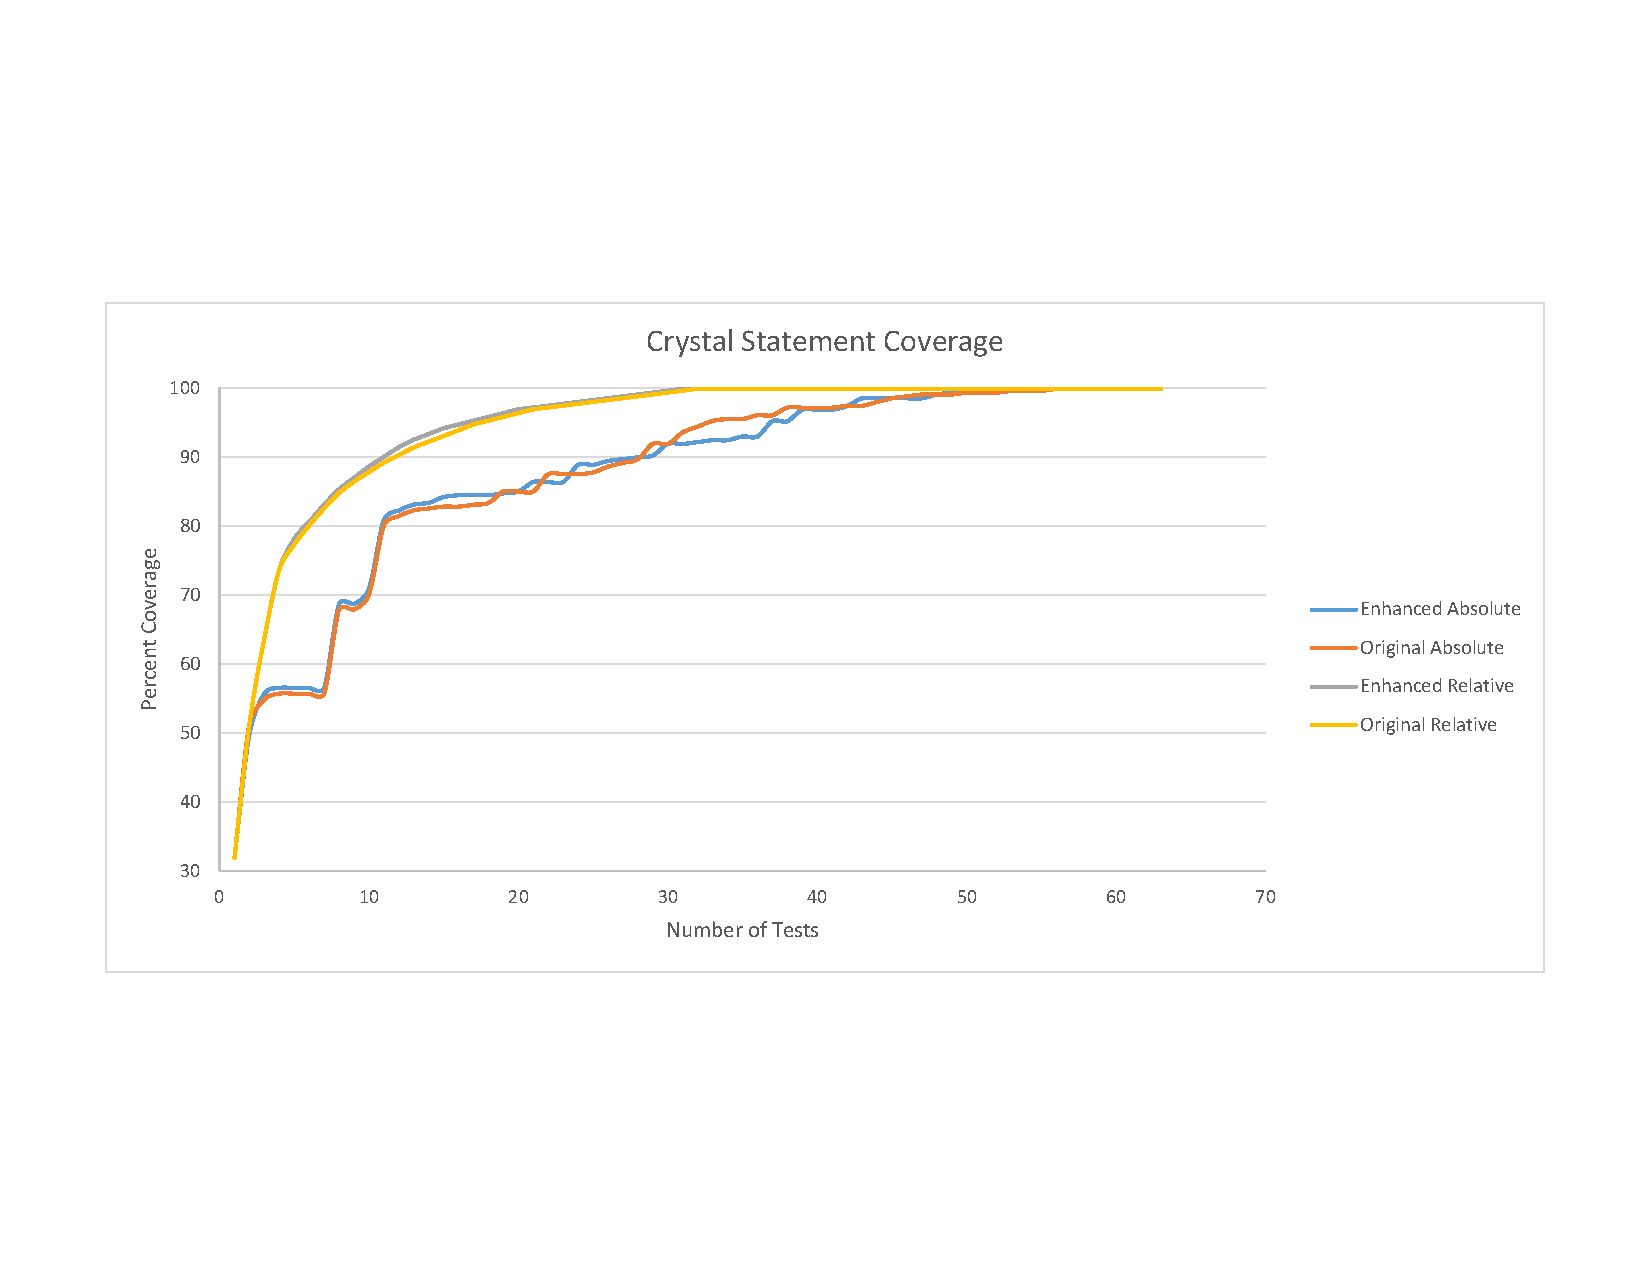
\includegraphics[scale=0.35]{crystal-coverage-figure}
{Crystal}
%\caption{tcas} \label{fig:p1}
\end{minipage}
\vspace{-6mm}
\caption{
    \label{fig:priocoverage}
Statement coverage results by each test prioritization technique on
our evaluation subject programs.
As shown in Table~\ref{tab:testprioresult}, the subject programs Synoptic
and XML-Security were omitted because none of the orders from their
nonenhanced orders revealed any dependent tests.
}
\end{figure}




\subsection{Dependence-Aware Test Prioritization}

All tests reveal the same results as being executed
in the default, unprioritized test suite in the prioritized
order produced by all enhanced, dependence-aware test
prioritization techniques. This is because when prioritizing
a test, the enhanced technique always checks whether
its depending tests have been executed before it or not. Thus,
the test dependence is preserved in the enhanced prioritized order.

We evaluate the effectiveness of the enhanced prioritized test suite
by measuring its coverage. Figure~\ref{fig:priocoverage}
shows the results. The test orders produced by the enhanced
test prioritization techniques achieves \textit{higher}
coverage \textit{faster} than the unenhanced test orders.
This was surprising because we expected a test order to achieve higher
coverage slower when we have to reorder it to preserve test dependence.
Yet the results we collected contradicted that.
Unlike the enhanced orders, dependent tests in the unenhanced orders
actually do not provide the coverage it does in the unprioritized test suite.
As an example, test $\mathit{a}$ may covers 50 statements when
executed in the unprioritized test suite. However because test
$\mathit{a}$ is dependent on test $\mathit{b}$ running before it,
if a test prioritization order does not have test $\mathit{b}$
running before test $\mathit{a}$, then test $\mathit{a}$ may only
cover a subset of the 50 statements it is expected to cover.
Common reasons for why our dependent tests achieved higher
coverage slower in our unenhanced orders was because of the
occurrences of events that disrupts the normal flow of
instructions and the different paths of execution taken for branches. 

\subsection{Dependence-Aware Test Selection}

\begin{table}
\centering
\setlength{\tabcolsep}{1.25\tabcolsep}
\begin{tabular}{|l|c|c|}
%\toprule
\hline
\textbf{Subject Program} & S1 (statement-level) & S2 (method-level)  \\
\hline
\multicolumn{3}{|l|}{}  \\
\multicolumn{3}{|l|}{\textbf{Human-written Test Suites}}  \\
\hline
\jt& 332 $\rightarrow$ 335 & 3233 $\rightarrow$ 3233 \\
XML Security& 70 $\rightarrow$ 83 & 71 $\rightarrow$ 84  \\
%\bottomrule
\hline
\textbf{Total} & 402 $\rightarrow$ 418 & 3304 $\rightarrow$ 3317 \\
\hline
%\textbf{Total}& &  & &  \\ 
%\hline
\end{tabular}
\caption{Results of evaluating the \selnum test selection techniques
in Table~\ref{tab:enhancetestsel} on four human-written unit test suites.
Each cell shows the number of selected tests.
As shown in Table~\ref{tab:testselresult}, the subject programs Crystal,
JFreeChart and Synoptic were omitted because none of the orders from their
nonenhanced orders revealed any dependent tests.
}
\label{tab:enhancedselresult}
\end{table}

All tests in the test subset selected by all test selection
techniques reveal the same result as in the default
test suite. Similar to the enhanced test prioritization
techniques, when selecting an affected test,
each enhanced test selection technique also checks whether
its depending tests have been selected and executed
before it in the selected test subset. Therefore,
the test dependence is always preserved.

We measure the size of the selected subset.  Table~\ref{tab:enhancedselresult}
shows the results. The enhanced techniques 
slightly increase the selected test subset by
less than  1\%.

\subsection{Dependence-Aware Test Parallelization}

\begin{table*}
\centering
\setlength{\tabcolsep}{1.25\tabcolsep}
\begin{tabular}{|l| l|l|l|l| l|l|l|l| l|l|l|l|}
%\toprule
\hline
\textbf{Subject Program} & \multicolumn{4}{|l|}{P1 (Original Order Parallelization)} &  \multicolumn{4}{|l|}{P2 (Random Parallelization)} & \multicolumn{4}{|l|}{P3 (Time-Minimized Parallelization)}\\
\cline{2-13}
& k=2 & k=4 & k=8 & k=16 & k=2 &k=4& k=8& k=16 & k=2 &k=4& k=8& k=16\\
\hline
\multicolumn{13}{|l|}{}  \\
\multicolumn{13}{|l|}{\textbf{Human-written Test Suites}}  \\
\hline
\jt& 3.47 & 1.97 & 1.84 & 1.80 & 2.83 & 2.61 & 1.92 & 1.80 & 2.20 & 2.11 & 1.38  & 1.79\\
XML Security& 1.45 & 1.89 & 2.48 & 5.72 & 1.56  & 2.35 & 4.02  & 4.25 & 2.56 & 2.82  & 4.38 & 6.00 \\
Crystal& 1.72  & 1.84  & 1.24  & 1.48  & 1.72 & 2.16& 1.72 & 1.04 & 2.12 & 1.34 & 1.33& 1.26\\
JFreechart&  1.33 & 1.26 & 1.15  & 1.27  & 1.44 & 1.28 & 1.30 & 1.22 & 1.46 & 1.31 & 1.31 & 1.40\\
%\bottomrule
\hline
\textbf{Average} & 1.99  & 1.74 & 1.67  & 2.57 & 1.89 & 2.10& 2.24 & 2.08 & 2.09 & 1.89 & 2.10 & 2.61\\
\hline
%\textbf{Total}& &  & &  \\ 
%\hline
\end{tabular}
\caption{
Results of evaluating the enhanced test parallelization techniques
on the subject programs. The numbers displayed in the table are
calculated from dividing the time cost to execute the enhanced
order by the time cost to execute the nonenhanced order.
As shown in Table~\ref{tab:testparresult}, the subject program Synoptic was
omitted because none of the orders from its nonenhanced orders revealed
any dependent tests.
\todo{show the slow}
}
\label{tab:enhancedparresult}
\end{table*}

By using the enhanced test parallelization techniques,
all tests scheduled on different machines reveal the
same results as being executed in the original test suite.

The major purpose of using test parallelization techniques is
to shorten the total test execution time. We measure the total
test execution time by recording the time taken by the slowest
machine. Table~\ref{tab:enhancedparresult} shows the
slowdown of each enhanced parallelization technique.
The slowdown varies across different techniques and test suites,
ranging from 1.67 to 2.61, on average. The slowdown is a result
of the increased amount of tests machines have to execute in
order to preserve test dependence. To elaborate, say test $\mathit{a}$
depends on test $\mathit{b}$ yet they were both scheduled
to be executed in different machines. In order for test $\mathit{a}$ to exhibit
the same behavior as it did in the unparallelized test suite, whichever
machine test $\mathit{a}$ is contained in will  have to have test
$\mathit{b}$ be added to it.


\subsection{Discussion}

\subsubsection{Threats to Validity}

There are several threats to the validity
of our experiments. 
%First, \dtexplain 
%only considers test dependencies arised
%from improper field access. It may not
%produce useful results for other types of
%test dependencies~\cite{}. 
First, the subject programs and the test suites
used to evaluate the enhanced testing techniques may
not be representative enough. We donot claim
our findings can be generalized to any subject
programs or test suites. Second,
when measuring the effectiveness of each enhanced
testing technique, we measure the test coverage
result, the size of the selected subset, and
the test execution time. We did not measure
Second,
\todo{evaluating on the test coverage, no
bug finding abilities yet.}

\subsubsection{Experimental Conclusions}

We have two chief findings. 
%\textbf{(1)} \dtexplain
%generates concise report to explain why
%test dependence arises, and such report
%helps developers to understand the root cause
%of test dependence.
\textbf{(1)} All enhanced downstream testing techniques
output consistent results on test suites
containing dependent tests. And \textbf{(2)}
The enhanced testing techniques have
little impact on the testing effectiveness.
